%%%%%%%%%%%%%%%%%%%%%%%%%%%%%% -*- Mode: Latex -*- %%%%%%%%%%%%%%%%%%%%%%%%%%%%
%% 09-02.tex --     ESEM 2009 Submission
%% Author          : Philip Johnson
%% Created On      : Wed Jan 07 14:06:37 2009
%% Last Modified By: Philip Johnson
%% Last Modified On: Wed Mar 04 10:06:18 2009
%% RCS: $Id$
%%%%%%%%%%%%%%%%%%%%%%%%%%%%%%%%%%%%%%%%%%%%%%%%%%%%%%%%%%%%%%%%%%%%%%%%%%%%%%%
%%   Copyright (C) 2009 
%%%%%%%%%%%%%%%%%%%%%%%%%%%%%%%%%%%%%%%%%%%%%%%%%%%%%%%%%%%%%%%%%%%%%%%%%%%%%%%
%% 
\documentclass{acm_proc_article-sp}

%
\def\sharedaffiliation{%
\end{tabular}
\begin{tabular}{c}}
%
\begin{document}

\title{I need more coverage, stat!  \\
Classroom experience with the Software ICU}

\numberofauthors{2} 

\author{
  \alignauthor Philip Johnson\\
  \email{johnson@hawaii.edu}
%
  \alignauthor Shaoxuan Zhang \\
  \email{sz@hawaii.edu}
%
  \sharedaffiliation
  \affaddr{Collaborative Software Development Laboratory}\\
  \affaddr{Department of Information and Computer Sciences}\\
  \affaddr{University of Hawaii}
}

\date{15 March 2008}

\maketitle
\begin{abstract}
One goal of the Hackystat Framework is to facilitate the teaching of
software metrics in classroom settings.  To that end, we have conducted
classroom evaluations in 2003, 2006, and 2008.  This paper reports in
detail on our most recent approach to teaching software metrics in the
classroom by way of an approach called the ``Software ICU''.  In this
approach, students learn about ten empirical project ``vital signs'' and
use the Hackystat Framework to put their students projects into a virtual
``intensive care unit'' where these vital signs can be assessed and
monitored.  We conducted a questionnaire-based evaluation that provides
insight into the strengths and weaknesses of this approach, how it compares
to previous approaches using the Hackystat Framework, and promising future
directions.
\end{abstract}

\category{D.2.8}{Software Engineering}{Metrics}[complexity measures, performance measures, software quality measures]

\section{Introduction}

Introducing students to software measurement in particular and empirical
software engineering in general is a challenging task.  

On the one hand, if one merely lectures about the literature, much of the
subtleties involved in the practice of collecting and analyzing process and
product data are lost.  An overly superficial presentation can lead
students to believe that software measurement is ``easy''. For example,
simply (1) collect complexity; (2) set a threshold using a published
reference such as \cite{Clark08}, and (3) require developers to ``fix'' any
classes that exceed the established threshold.  The problem is that
individual metrics never capture the spectrum of trade-offs implicit in a
design. For example, a natural result of performance optimization on a
section of code is an increase in complexity (and coupling). Measurements
on such classes might exceed thresholds for important reasons.  Without
such real world grounding, such students could grow up to be the
stereotypical process improvement managers who impose ``best practices''
for measurement and analysis without understanding the potential for
misinterpretation and, ultimately, measurement dysfunction \cite{Austin96}.

On the other hand, requiring students to gather and analyze measurements
themselves can potentially lead students to believe that measurement is too
``hard''.  For example, while the Personal Software Process
\cite{Humphrey95} provides a well structured approach to data gathering and
analysis by students, independent research reveals a number of problems
including high overhead \cite{csdl2-01-12}, data quality \cite{csdl-98-13},
and low adoption \cite{Borstler02}.  Students introduced to metrics via the
PSP (or its successor, the Team Software Process) can easily form the
impression that software measurement imposes too much overhead for (at the very
least) ``agile'' software development situations.

For the past five years, one research thrust of the Hackystat Framework has
been to explore the issues involved in teaching software measurement in a
classroom setting.  Hackystat provides a pedagogical middle ground between
excessively high overhead approaches like the PSP/TSP and excessively low
overhead approaches like literature review.  Extensive automation of both
data collection and analysis lowers the overhead required to give students
practical experience with measurement, while creating opportunities to
understand some of the nuances involved with analysis, presentation, and
interpretation.

In this paper, we present the results of a case study experiment we
performed in the Fall of 2008 in which we used the metaphor of a medical
intensive care unit (ICU) to explain and motivate the use of metrics in
software development.  We built a new user interface for metric data called
the ``Software ICU'' that is similar in many ways to a medical ICU
monitoring device.  Just as a medical ICU automatically gathers vital signs
of patients such as heart rate and respiration in order to detect changes
in health, our software ICU automatically monitors the process and product
``vital signs'' of its software ``patients''---in this case, the student
teams and the projects they were developing.  Just as a medical ICU
generates alarms when a vital sign falls outside a established range for
normalacy, our software ICU can color metrics as red, yellow, or green to
indicate problematic, unstable, or healthy software vital signs. 

We collected two types of data: an online questionnaire that the students
filled out at the end of the study, and system-generated log data that
collected all student interactions with the Software ICU.  Our results
provide evidence that, in general, the Software ICU is currently the most
effective Hackystat-based approach to teaching students about process and
product measurement.  Student feedback indicates that the overhead involved
in data collection and analysis was acceptably low, and almost all of the
students found the data to be useful, although students found some ``vital
signs'' to be more useful than others. Most students believed that the
Software ICU would be feasible for use in professional situations.  The log
data provided independent confirmation of the usage of the system, as the
majority of students invoked the Software ICU from 20 to 40 times per week
during the course of the study.

The remainder of the paper is organized as follows.  Section
\ref{sec:related} presents related work.  Section \ref{sec:icu} provides a
brief overview of the system. Section \ref{sec:evaluation} presents the
case study design and its results.  Section \ref{sec:conclusions} presents
our conclusions and future directions.

\section {Related Work}
\label{sec:related}

Perhaps the most extensively studied curriculum for measure\-ment-based
software engineering is the Personal Software Process \cite{Humphrey95} and
the Team Software Process \cite{Humphrey00}.  Both of these approaches
require students to develop a series of software projects, typically six to
eight during a single semester.  Both process and product measures are
gathered about each project, and the measurements become increasingly
detailed as the semester proceeeds. After the first three projects are
completed, the students can use the completed projects as historical data
to support quality improvement (by identifying repeated types of defects)
and estimation (through simple linear regression).  The PSP/TSP methods
enjoy strong support from the Software Engineering Institute, and they have
a published a number of case studies indicating success in a classroom setting. 

Conn developed a metrics-based software engineering course called the 
IS Integrated Capstone Project \cite{Conn04}.  The metrics were closely aligned
with the PSP/TSP format, though some of the process constraints were relaxed. 

Robillard designed a project-based course in which students were required
to fill out logs that specified the time spent on various activities
\cite{Robillard98}.  No automation of data collection was supported in this
approach.  Barry and Norris created Project ClockIt to facilitate the
profiling of student software development practices \cite{Barry05}.  Unlike
the manual log-based time data collection used by Robillard, Project
ClockIt provides automated collection of time data through a plugin to the
student's IDE.

Williams created the Open Seminar module on Software Engineering to collect
curriculum resources on software engineering.  There is a module on
object-oriented metrics, and several modules related to Agile practices.  

The metaphor of ``software health'' is not unique to this research.
Organizations concerned with expensive, life-critical hardware-software
systems have long been concerned with assessing their health at run-time
and potentially recovering from unhealthy states \cite{Hadden00,
Thai01}. Our approach focuses on the health of the system during
development, not execution.

The research presented in this paper is the third case study we have
performed on measurement collection and analysis in a classroom setting
using Hackystat.  In 2003, we performed our first case study in which we used an
early version of Hackystat to automate data collection and analysis and
used a survey to assess student reactions \cite{csdl2-03-12}.  In this
study, we found that students encountered significant problems during the
installation of the system, that analyses were somewhat useful, and that
privacy and platform issues were thought to be significant issues in a
professional setting.

In 2006, we performed a partial replication of the first case study.  It
was a partial replication because the Hackystat system had significantly
evolved since 2003 and so we changed some of the evaluation questions to
better suit the current needs.  On the positive side, students reported
less problems during installation, reflecting the work we had done since
2003 on a client-side installer.  On the negative side, the much larger set
of analyses available in 2006 impacted on the usability of the system:
students were more confused about which analyses to use and how to
interpret the results.

For these and other reasons, we decided in 2007 to begin a major
re-implementation of Hackystat as a service-oriented architecture
\cite{csdl2-09-07}. The new system provided us with the ability to redesign
the user interface to Hackystat.  Instead of a single, monolithic user
interface with a predefined look and feel, the new architecture allowed us
to implement multiple, special purpose interfaces using a wide variety of
UI technologies.  

In 2008, we finished the re-implementation of the basic facilities as well
as a new approach to multi-project metrics visualization called Portfolio
Analysis.  In Fall of 2008, we performed a third case study. This time, we used 
the metaphor of the ``Software ICU'', as discussed next.

\section{From Medical to Software ICU}
\label{sec:icu}

Medical intensive care units feature automatic and continuous monitoring of
patient vital signs.  The four fundamental medical vital signs are
temperature, heart rate, blood pressure and respiration.  Other vital signs
may be monitored depending upon the particulars of a patient condition.

\begin{figure}[ht]
  \center
  \includegraphics[width=0.4\textwidth]{micu-screen.eps}
  \caption{An example Medical ICU monitoring device}
  \label{fig:micu}
\end{figure} 

Figure \ref{fig:micu} illustrates a sample medical ICU display unit. For
each of the four fundamental vital signs, the interface shows both its
current numeric value as well as a graph showing its recent history.  

Each of these vital signs has a ``normal range of behavior'', and the
monitoring unit can raise an alarm when any of the patient's vital signs departs
from its normal range of behavior.

Vital signs are interesting because: (a) in a ``healthy'' patient, they are
normal or improving; (b) change in one vital sign may or may not be
significant; (c) change in multiple vital signs is almost certainly
significant, particularly if more than one are outside their normal range.

Translating medical ICU practices to the context of a software engineering
class required us to redefine ``health'', ``vital signs'', ``normal range''
and the ICU monitoring user interface in terms useful to students and their
software development projects.

We defined a ``healthy'' development project as satisfying three high-level
characteristics: high efficiency (software development proceeds ``as fast
as possible, but no faster''); high effectiveness (effort is focused on the
most important issues, with minimal rework); and high quality (software
satisfies user needs; software can be easily installed, adapted, and
maintained).

We then presented a set of simple practices that, if followed, we claimed
would raise the probability of their projects being ``healthy''.  These
included: everyone works consistently; everyone contributes equally; code
is committed consistently; progress is regular; quality remains high; no
last minute rush to finish.  These development practices are analogous to
life-style behaviors like ``eat right'', ``get enough sleep'' and
``exercise regularly'' that generally facilitate (but, of course, do not
guarantee) good health in a patient.

Next, we presented ten software ``vital signs'': coverage, complexity,
coupling, churn, code issues, builds, commits, unit tests, size, and dev
time. Through a combination of Hackystat sensors and the Hudson continuous
integration system, these 10 vital signs could be automatically and
continously collected for their projects.

For each software vital sign, we then presented its ``normal range of
behavior''.  For example, for the coupling vital sign to be considered
``healthy'', its current value should be above 90\% and the trend in
coverage over time should be stable or increasing.  For the commit vital
sign to be considered normal, at least 50\% of the team members should have
committed, and there should be commits on at least 50\% of the days in the
project interval.  For one of the vital signs, ``size'', we stated that
there is no simple way of assessing its nnormal range of behavior, though
it still provides some value in understanding project health.

Unlike a medical ICU, where there is literally hundreds of years of medical
research establishing both the importance of the four fundamental vital
signs and their normal range of behaviors, no such consensus exists in
software engineering on what would constitute ``fundamental'' software
vital signs or their normal range of behavior.  Thus, our selection of
software vital signs and their normal range of behaviors are actually
research hypotheses.  We designed the case study to elicit evidence
regarding the appropriateness of these vital signs and our proposed normal
range of behaviors.

Finally, we presented the user interface to the Software ICU. A portion of
this user interface appears in Figure \ref{fig:sicu}.

\begin{figure*}[ht]
  \center
  \includegraphics[width=0.8\textwidth]{portfolio-2008.eps}
  \caption{An example Software ICU analysis}
  \label{fig:sicu}
\end{figure*} 

Each row in the Software ICU interface provides information about one
software project, or ``patient''.  Each column presents information about
one vital sign. Similar to the medical ICU, the software ICU presents both
the most recent numeric value as well as the recent trend in value for each
vital sign.

We decided to represent ``normal range in behavior'' by independently
coloring the trend line and the most recent value as green, yellow, or red
depending upon whether the value was ``healthy'', ``unstable'', or
``unhealthy''.  We did not implement ``alarms'', such as emails or text
messages to team members if a vital sign turns red, although this is a
possible future extension.  Instead, it was the responsibility of the
students to invoke the software ICU regularly in order to monitor the
health of their project.  During the case study, we collected log data to
gather evidence about whether they in fact did this monitoring.

To help make the vital sign actionable, the Software ICU supported ``drill
down'' for trend data.  Figure \ref{fig:telemetry} shows one such drilldown
that reveals that only one of the four members of the project was doing the
vast majority of commits.

\begin{figure*}[ht]
  \center
  \includegraphics[width=0.8\textwidth]{telemetry-screen.eps}
  \caption{A drill-down showing commit telemetry}
  \label{fig:telemetry}
\end{figure*} 

The measurements underlying the Software ICU were collected automatically
through two mechanisms. First, the students installed Hackystsat sensors
into their IDE (Eclipse) and build system (Ant) which sent process
metrics regarding their development activities.  Second, their projects
used the Hudson system to perform continuous integration, which meant that
after each commit of their code, the system would be automatically built
and tested.  The Hudson system was also configured to automatically gather
certain product metrics such as coverage, coupling, and complexity.

\section{Evaluation}
\label{sec:evaluation}

Our case study was focused on addressing the following research questions: 
\begin{itemize}
\item What are the strengths and weaknesses of the medical ICU metaphor for 
teaching software measurement in a classroom setting? 
\item How appropriate were our choices of ``vital signs''?
\item How effective were our algorithms for coloring the vital signs? 
\item How does this approach compare to previous uses of Hackystat to teach software metrics
in a classroom setting? 
\end{itemize}

The study involved 18 students from a senior-level undergraduate software
engineering course at the University of Hawaii from Fall, 2008. This course
teaches software engineering in the context of open source development
using the Java programming language.  The first several weeks are concerned
with basic tools and technologies, including interactive development
environments, coding standards, static analysis tools for quality
assurance, build systems, configuration management, and software review.
The course taught these concepts in the context of a semester project,
which in this semester was a web application for automated tracking and
notification of library book due dates.  We introduced the Software ICU
during the final five weeks of the semester, and the students used it for
two increments of development.

During the final week of the semester, we made available to them an online
survey containing 17 questions.  These questions asked the students their
opinions regarding the overhead involved with installing sensors, problems
they encountered, frequency of use of the system, the vital signs they
found useful, and the utility of the system and its appropriateness for an
industrial setting.  A companion technical report to this paper provides
the full text of the survey \cite{csdl2-09-03}.

Students picked a random string from a hat and provided the string and
their name to a graduate student researcher.  They used this string to
identify themselves in the online questionnaire.  They were told that the
instructor for the class would not know their responses, but that the
graduate student would provide the names of all students completing the
questionnaire to the instructor, who would then award extra credit for
participation.  This approach incentivized participation, provided some
level of anonymity to the students, prevented non-students from completing
the survey, prevented multiple responses by a single student, and allowed
the graduate student to compare the log data for that student to their
survey responses in order to cross-validate some of their answers. All but 
one of the students in the class completed the questionnaire.

For complete details on the responses and our analysis of the results, we 
refer you to the companion technical report \cite{csdl2-09-03}.  Space limitations 
require us to present only selected findings. 



\section{Conclusions and future directions}
\label{sec:conclusions}

Remember to compare to dashboards. 



Where we will go next.

\section{Acknowledgments}

We will acknowledge some folks here.

\bibliographystyle{abbrv}
\bibliography{csdl-trs,hackystat,psp}  

%% In this paper, we present the results of our third partial replication with
%% yet another redesigned version of Hackystat in the Fall of 2008.  One major
%% change in our current approach is the complete abandonment of terminology
%% like ``software measurement'' or ``metrics'' as the pedagogical focus.
%% Instead, we present the material through the metaphor of a medical
%% intensive care unit (ICU).  Instead of ``metrics'', we taught the students
%% about how to acquire software ``vital signs''.  The goal of vital sign
%% collection was to assess whether the ``patient'' (software system under
%% development) was ``healthy'' or ``sick''.  The user interface was modeled
%% after a medical ICU vital sign monitor, with the ability to display both
%% the current value as well as the trends (heartbeats) over time.  Just as a
%% vital sign monitor can be set with alarms, the Software ICU monitor can be
%% configured with thresholds to color the current value or trend either red,
%% yellow, or green.  Finally, just as an ICU supports multiple patients, our
%% Software ICU can show the status of multiple projects simultaneously,
%% supporting ease of comparative evaluation.

\end{document}

